\documentclass[twoside]{book}

% Packages required by doxygen
\usepackage{fixltx2e}
\usepackage{calc}
\usepackage{doxygen}
\usepackage{graphicx}
\usepackage[utf8]{inputenc}
\usepackage{makeidx}
\usepackage{multicol}
\usepackage{multirow}
\PassOptionsToPackage{warn}{textcomp}
\usepackage{textcomp}
\usepackage[nointegrals]{wasysym}
\usepackage[table]{xcolor}

% Font selection
\usepackage[T1]{fontenc}
\usepackage{mathptmx}
\usepackage[scaled=.90]{helvet}
\usepackage{courier}
\usepackage{amssymb}
\usepackage{sectsty}
\renewcommand{\familydefault}{\sfdefault}
\allsectionsfont{%
  \fontseries{bc}\selectfont%
  \color{darkgray}%
}
\renewcommand{\DoxyLabelFont}{%
  \fontseries{bc}\selectfont%
  \color{darkgray}%
}
\newcommand{\+}{\discretionary{\mbox{\scriptsize$\hookleftarrow$}}{}{}}

% Page & text layout
\usepackage{geometry}
\geometry{%
  a4paper,%
  top=2.5cm,%
  bottom=2.5cm,%
  left=2.5cm,%
  right=2.5cm%
}
\tolerance=750
\hfuzz=15pt
\hbadness=750
\setlength{\emergencystretch}{15pt}
\setlength{\parindent}{0cm}
\setlength{\parskip}{0.2cm}
\makeatletter
\renewcommand{\paragraph}{%
  \@startsection{paragraph}{4}{0ex}{-1.0ex}{1.0ex}{%
    \normalfont\normalsize\bfseries\SS@parafont%
  }%
}
\renewcommand{\subparagraph}{%
  \@startsection{subparagraph}{5}{0ex}{-1.0ex}{1.0ex}{%
    \normalfont\normalsize\bfseries\SS@subparafont%
  }%
}
\makeatother

% Headers & footers
\usepackage{fancyhdr}
\pagestyle{fancyplain}
\fancyhead[LE]{\fancyplain{}{\bfseries\thepage}}
\fancyhead[CE]{\fancyplain{}{}}
\fancyhead[RE]{\fancyplain{}{\bfseries\leftmark}}
\fancyhead[LO]{\fancyplain{}{\bfseries\rightmark}}
\fancyhead[CO]{\fancyplain{}{}}
\fancyhead[RO]{\fancyplain{}{\bfseries\thepage}}
\fancyfoot[LE]{\fancyplain{}{}}
\fancyfoot[CE]{\fancyplain{}{}}
\fancyfoot[RE]{\fancyplain{}{\bfseries\scriptsize Generated on Wed Mar 7 2018 15\+:01\+:01 for Banking Test by Doxygen }}
\fancyfoot[LO]{\fancyplain{}{\bfseries\scriptsize Generated on Wed Mar 7 2018 15\+:01\+:01 for Banking Test by Doxygen }}
\fancyfoot[CO]{\fancyplain{}{}}
\fancyfoot[RO]{\fancyplain{}{}}
\renewcommand{\footrulewidth}{0.4pt}
\renewcommand{\chaptermark}[1]{%
  \markboth{#1}{}%
}
\renewcommand{\sectionmark}[1]{%
  \markright{\thesection\ #1}%
}

% Indices & bibliography
\usepackage{natbib}
\usepackage[titles]{tocloft}
\setcounter{tocdepth}{3}
\setcounter{secnumdepth}{5}
\makeindex

% Hyperlinks (required, but should be loaded last)
\usepackage{ifpdf}
\ifpdf
  \usepackage[pdftex,pagebackref=true]{hyperref}
\else
  \usepackage[ps2pdf,pagebackref=true]{hyperref}
\fi
\hypersetup{%
  colorlinks=true,%
  linkcolor=blue,%
  citecolor=blue,%
  unicode%
}

% Custom commands
\newcommand{\clearemptydoublepage}{%
  \newpage{\pagestyle{empty}\cleardoublepage}%
}


%===== C O N T E N T S =====

\begin{document}

% Titlepage & ToC
\hypersetup{pageanchor=false,
             bookmarks=true,
             bookmarksnumbered=true,
             pdfencoding=unicode
            }
\pagenumbering{roman}
\begin{titlepage}
\vspace*{7cm}
\begin{center}%
{\Large Banking Test }\\
\vspace*{1cm}
{\large Generated by Doxygen 1.8.8}\\
\vspace*{0.5cm}
{\small Wed Mar 7 2018 15:01:01}\\
\end{center}
\end{titlepage}
\clearemptydoublepage
\tableofcontents
\clearemptydoublepage
\pagenumbering{arabic}
\hypersetup{pageanchor=true}

%--- Begin generated contents ---
\chapter{Class Index}
\section{Class List}
Here are the classes, structs, unions and interfaces with brief descriptions\+:\begin{DoxyCompactList}
\item\contentsline{section}{\hyperlink{classPCO_1_1Athlete}{P\+C\+O.\+Athlete} \\*\hyperlink{classPCO_1_1Athlete}{Athlete} class to input individual's personal information and events to partake in }{\pageref{classPCO_1_1Athlete}}{}
\item\contentsline{section}{\hyperlink{classPCO_1_1Database}{P\+C\+O.\+Database} \\*D\+E\+P\+R\+E\+C\+A\+T\+E\+D!!! \hyperlink{classPCO_1_1Database}{Database} S\+U\+B\+S\+Y\+S\+T\+E\+M houses all the information of the Winter Olympics }{\pageref{classPCO_1_1Database}}{}
\item\contentsline{section}{\hyperlink{classPCO_1_1Event}{P\+C\+O.\+Event} \\*\hyperlink{classPCO_1_1Event}{Event} class is the superclass of all the 2 event types and 6 specific events }{\pageref{classPCO_1_1Event}}{}
\item\contentsline{section}{\hyperlink{interfacePCO_1_1Event_1_1eventInheritance}{P\+C\+O.\+Event.\+event\+Inheritance} }{\pageref{interfacePCO_1_1Event_1_1eventInheritance}}{}
\item\contentsline{section}{\hyperlink{classPCO_1_1FigureSkating}{P\+C\+O.\+Figure\+Skating} \\*\hyperlink{classPCO_1_1FigureSkating}{Figure\+Skating} class is the superclass of the 3 \hyperlink{classPCO_1_1FigureSkating}{Figure\+Skating} events }{\pageref{classPCO_1_1FigureSkating}}{}
\item\contentsline{section}{\hyperlink{interfacePCO_1_1FigureSkating_1_1fsInheritance}{P\+C\+O.\+Figure\+Skating.\+fs\+Inheritance} }{\pageref{interfacePCO_1_1FigureSkating_1_1fsInheritance}}{}
\item\contentsline{section}{\hyperlink{classPCO_1_1IceDance}{P\+C\+O.\+Ice\+Dance} \\*\hyperlink{classPCO_1_1IceDance}{Ice\+Dance} class is one of the 3 \hyperlink{classPCO_1_1FigureSkating}{Figure\+Skating} events }{\pageref{classPCO_1_1IceDance}}{}
\item\contentsline{section}{\hyperlink{classPCO_1_1Judge}{P\+C\+O.\+Judge} \\*\hyperlink{classPCO_1_1Judge}{Judge} class houses and disperses all the qualified judges }{\pageref{classPCO_1_1Judge}}{}
\item\contentsline{section}{\hyperlink{classPCO_1_1MainClass}{P\+C\+O.\+Main\+Class} }{\pageref{classPCO_1_1MainClass}}{}
\item\contentsline{section}{\hyperlink{classPCO_1_1PairSkating}{P\+C\+O.\+Pair\+Skating} \\*\hyperlink{classPCO_1_1PairSkating}{Pair\+Skating} class is one of the 3 \hyperlink{classPCO_1_1FigureSkating}{Figure\+Skating} events }{\pageref{classPCO_1_1PairSkating}}{}
\item\contentsline{section}{\hyperlink{classPCO_1_1Registration}{P\+C\+O.\+Registration} \\*\hyperlink{classPCO_1_1Registration}{Registration} class registers Teams and Athletes }{\pageref{classPCO_1_1Registration}}{}
\item\contentsline{section}{\hyperlink{classPCO_1_1Rink}{P\+C\+O.\+Rink} \\*\hyperlink{classPCO_1_1Rink}{Rink} class is the physical area in which events are held }{\pageref{classPCO_1_1Rink}}{}
\item\contentsline{section}{\hyperlink{classPCO_1_1Schedule}{P\+C\+O.\+Schedule} \\*\hyperlink{classPCO_1_1Schedule}{Schedule} class is the organization of athletes and events }{\pageref{classPCO_1_1Schedule}}{}
\item\contentsline{section}{\hyperlink{classPCO_1_1Scoring}{P\+C\+O.\+Scoring} \\*\hyperlink{classPCO_1_1Scoring}{Scoring} class manages the official scores/times recorded by the judges }{\pageref{classPCO_1_1Scoring}}{}
\item\contentsline{section}{\hyperlink{classPCO_1_1SingleSkating}{P\+C\+O.\+Single\+Skating} \\*\hyperlink{classPCO_1_1SingleSkating}{Single\+Skating} class is one of the 3 \hyperlink{classPCO_1_1FigureSkating}{Figure\+Skating} events }{\pageref{classPCO_1_1SingleSkating}}{}
\item\contentsline{section}{\hyperlink{classPCO_1_1SpeedSkating}{P\+C\+O.\+Speed\+Skating} \\*\hyperlink{classPCO_1_1SpeedSkating}{Speed\+Skating} class is the superclass of the 3 \hyperlink{classPCO_1_1SpeedSkating}{Speed\+Skating} events }{\pageref{classPCO_1_1SpeedSkating}}{}
\item\contentsline{section}{\hyperlink{classPCO_1_1SS1000m}{P\+C\+O.\+S\+S1000m} \\*\hyperlink{classPCO_1_1SS1000m}{S\+S1000m} is one of the 3 \hyperlink{classPCO_1_1SpeedSkating}{Speed\+Skating} events }{\pageref{classPCO_1_1SS1000m}}{}
\item\contentsline{section}{\hyperlink{classPCO_1_1SS1500m}{P\+C\+O.\+S\+S1500m} \\*\hyperlink{classPCO_1_1SS1500m}{S\+S1500m} is one of the 3 \hyperlink{classPCO_1_1SpeedSkating}{Speed\+Skating} events }{\pageref{classPCO_1_1SS1500m}}{}
\item\contentsline{section}{\hyperlink{classPCO_1_1SS500m}{P\+C\+O.\+S\+S500m} \\*\hyperlink{classPCO_1_1SS500m}{S\+S500m} is one of the 3 \hyperlink{classPCO_1_1SpeedSkating}{Speed\+Skating} events }{\pageref{classPCO_1_1SS500m}}{}
\item\contentsline{section}{\hyperlink{interfacePCO_1_1SpeedSkating_1_1ssInheritance}{P\+C\+O.\+Speed\+Skating.\+ss\+Inheritance} }{\pageref{interfacePCO_1_1SpeedSkating_1_1ssInheritance}}{}
\item\contentsline{section}{\hyperlink{classPCO_1_1Team}{P\+C\+O.\+Team} \\*\hyperlink{classPCO_1_1Team}{Team} class to house the team name }{\pageref{classPCO_1_1Team}}{}
\end{DoxyCompactList}

\chapter{File Index}
\section{File List}
Here is a list of all files with brief descriptions\+:\begin{DoxyCompactList}
\item\contentsline{section}{\hyperlink{Class1_8cs}{Class1.\+cs} }{\pageref{Class1_8cs}}{}
\item\contentsline{section}{\hyperlink{Display_8cs}{Display.\+cs} }{\pageref{Display_8cs}}{}
\item\contentsline{section}{\hyperlink{Display_8Designer_8cs}{Display.\+Designer.\+cs} }{\pageref{Display_8Designer_8cs}}{}
\item\contentsline{section}{\hyperlink{Event_8cs}{Event.\+cs} }{\pageref{Event_8cs}}{}
\item\contentsline{section}{\hyperlink{Event_8Designer_8cs}{Event.\+Designer.\+cs} }{\pageref{Event_8Designer_8cs}}{}
\item\contentsline{section}{\hyperlink{Form1_8cs}{Form1.\+cs} }{\pageref{Form1_8cs}}{}
\item\contentsline{section}{\hyperlink{Form1_8Designer_8cs}{Form1.\+Designer.\+cs} }{\pageref{Form1_8Designer_8cs}}{}
\item\contentsline{section}{\hyperlink{Judge_8cs}{Judge.\+cs} }{\pageref{Judge_8cs}}{}
\item\contentsline{section}{\hyperlink{Judge_8Designer_8cs}{Judge.\+Designer.\+cs} }{\pageref{Judge_8Designer_8cs}}{}
\item\contentsline{section}{\hyperlink{Program_8cs}{Program.\+cs} }{\pageref{Program_8cs}}{}
\item\contentsline{section}{\hyperlink{Registration_8cs}{Registration.\+cs} }{\pageref{Registration_8cs}}{}
\item\contentsline{section}{\hyperlink{Registration_8Designer_8cs}{Registration.\+Designer.\+cs} }{\pageref{Registration_8Designer_8cs}}{}
\item\contentsline{section}{\hyperlink{Team_8cs}{Team.\+cs} }{\pageref{Team_8cs}}{}
\item\contentsline{section}{\hyperlink{Team_8Designer_8cs}{Team.\+Designer.\+cs} }{\pageref{Team_8Designer_8cs}}{}
\end{DoxyCompactList}

\chapter{Class Documentation}
\hypertarget{classBank}{\section{Bank Class Reference}
\label{classBank}\index{Bank@{Bank}}
}


{\ttfamily \#include $<$Bank.\+h$>$}



Collaboration diagram for Bank\+:\nopagebreak
\begin{figure}[H]
\begin{center}
\leavevmode
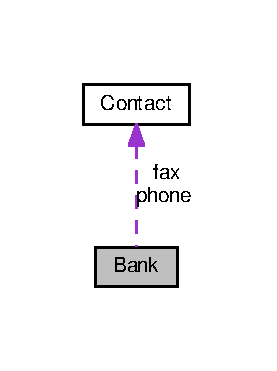
\includegraphics[width=133pt]{classBank__coll__graph}
\end{center}
\end{figure}
\subsection*{Public Member Functions}
\begin{DoxyCompactItemize}
\item 
\hyperlink{classBank_a95972e189e85e1a572348811a8bf0d57}{Bank} ()
\item 
\hyperlink{classBank_a65e1c804648aeb2d180d6e54c92ebc20}{Bank} (int \hyperlink{classID}{I\+D}, \hyperlink{classContact}{Contact} phone\+Num, \hyperlink{classContact}{Contact} fax\+Num)
\item 
void \hyperlink{classBank_ab4a84d64ec7d51762d5fd0affa900f8c}{display} ()
\end{DoxyCompactItemize}
\subsection*{Private Attributes}
\begin{DoxyCompactItemize}
\item 
int \hyperlink{classBank_a06dfa13f15b434d0bd135229d8b71843}{bank\+\_\+\+I\+D}
\item 
\hyperlink{classContact}{Contact} \hyperlink{classBank_a27aa9c6b6d1884365910d118dcf2b5c6}{phone}
\item 
\hyperlink{classContact}{Contact} \hyperlink{classBank_a2289ec7adf9926d419db85a706d5e7d9}{fax}
\end{DoxyCompactItemize}


\subsection{Constructor \& Destructor Documentation}
\hypertarget{classBank_a95972e189e85e1a572348811a8bf0d57}{\index{Bank@{Bank}!Bank@{Bank}}
\index{Bank@{Bank}!Bank@{Bank}}
\subsubsection[{Bank}]{\setlength{\rightskip}{0pt plus 5cm}Bank\+::\+Bank (
\begin{DoxyParamCaption}
{}
\end{DoxyParamCaption}
)}}\label{classBank_a95972e189e85e1a572348811a8bf0d57}
\hypertarget{classBank_a65e1c804648aeb2d180d6e54c92ebc20}{\index{Bank@{Bank}!Bank@{Bank}}
\index{Bank@{Bank}!Bank@{Bank}}
\subsubsection[{Bank}]{\setlength{\rightskip}{0pt plus 5cm}Bank\+::\+Bank (
\begin{DoxyParamCaption}
\item[{int}]{I\+D, }
\item[{{\bf Contact}}]{phone\+Num, }
\item[{{\bf Contact}}]{fax\+Num}
\end{DoxyParamCaption}
)}}\label{classBank_a65e1c804648aeb2d180d6e54c92ebc20}


\subsection{Member Function Documentation}
\hypertarget{classBank_ab4a84d64ec7d51762d5fd0affa900f8c}{\index{Bank@{Bank}!display@{display}}
\index{display@{display}!Bank@{Bank}}
\subsubsection[{display}]{\setlength{\rightskip}{0pt plus 5cm}void Bank\+::display (
\begin{DoxyParamCaption}
{}
\end{DoxyParamCaption}
)}}\label{classBank_ab4a84d64ec7d51762d5fd0affa900f8c}


\subsection{Member Data Documentation}
\hypertarget{classBank_a06dfa13f15b434d0bd135229d8b71843}{\index{Bank@{Bank}!bank\+\_\+\+I\+D@{bank\+\_\+\+I\+D}}
\index{bank\+\_\+\+I\+D@{bank\+\_\+\+I\+D}!Bank@{Bank}}
\subsubsection[{bank\+\_\+\+I\+D}]{\setlength{\rightskip}{0pt plus 5cm}int Bank\+::bank\+\_\+\+I\+D\hspace{0.3cm}{\ttfamily [private]}}}\label{classBank_a06dfa13f15b434d0bd135229d8b71843}
\hypertarget{classBank_a2289ec7adf9926d419db85a706d5e7d9}{\index{Bank@{Bank}!fax@{fax}}
\index{fax@{fax}!Bank@{Bank}}
\subsubsection[{fax}]{\setlength{\rightskip}{0pt plus 5cm}{\bf Contact} Bank\+::fax\hspace{0.3cm}{\ttfamily [private]}}}\label{classBank_a2289ec7adf9926d419db85a706d5e7d9}
\hypertarget{classBank_a27aa9c6b6d1884365910d118dcf2b5c6}{\index{Bank@{Bank}!phone@{phone}}
\index{phone@{phone}!Bank@{Bank}}
\subsubsection[{phone}]{\setlength{\rightskip}{0pt plus 5cm}{\bf Contact} Bank\+::phone\hspace{0.3cm}{\ttfamily [private]}}}\label{classBank_a27aa9c6b6d1884365910d118dcf2b5c6}


The documentation for this class was generated from the following files\+:\begin{DoxyCompactItemize}
\item 
\hyperlink{Bank_8h}{Bank.\+h}\item 
\hyperlink{Bank_8cpp}{Bank.\+cpp}\end{DoxyCompactItemize}

\hypertarget{classContact}{\section{Contact Class Reference}
\label{classContact}\index{Contact@{Contact}}
}


{\ttfamily \#include $<$Contact.\+h$>$}

\subsection*{Public Member Functions}
\begin{DoxyCompactItemize}
\item 
\hyperlink{classContact_ae39444f378e6de7fd6c3e60981949af5}{Contact} ()
\item 
\hyperlink{classContact_a90c224b7814afe056da1a339eeab928a}{Contact} (int area, int prefix, int suffix)
\item 
void \hyperlink{classContact_a531320e14eaa9bebf67d46fe97e46f9f}{set\+Area} (int area)
\item 
void \hyperlink{classContact_a172dccd347efe81bc7c844a0bb24502f}{set\+Prefix} (int prefix)
\item 
void \hyperlink{classContact_a0e762158350dfc8b22e9446d2820c05b}{set\+Suffix} (int suffix)
\item 
int \hyperlink{classContact_ad8ad13da697275f7243a21132f4d7224}{get\+Area} ()
\item 
int \hyperlink{classContact_afb68a34353910b2a7fb012f2c3c665c6}{get\+Prefix} ()
\item 
int \hyperlink{classContact_a36b4490ede1fe1114c25ecd68ba29ab1}{get\+Suffix} ()
\item 
void \hyperlink{classContact_a1a7b491fba3111a679bfae344d75d19d}{display} ()
\end{DoxyCompactItemize}
\subsection*{Private Attributes}
\begin{DoxyCompactItemize}
\item 
int \hyperlink{classContact_a9982efa21fdf3aa80ecb27fca50c1112}{area\+Code}
\item 
int \hyperlink{classContact_af88818b83e23babeeaccadbd957c5b3a}{prefix\+Num}
\item 
int \hyperlink{classContact_a741fc49c27f513429795c99b07bceae1}{suffix\+Num}
\end{DoxyCompactItemize}


\subsection{Constructor \& Destructor Documentation}
\hypertarget{classContact_ae39444f378e6de7fd6c3e60981949af5}{\index{Contact@{Contact}!Contact@{Contact}}
\index{Contact@{Contact}!Contact@{Contact}}
\subsubsection[{Contact}]{\setlength{\rightskip}{0pt plus 5cm}Contact\+::\+Contact (
\begin{DoxyParamCaption}
{}
\end{DoxyParamCaption}
)}}\label{classContact_ae39444f378e6de7fd6c3e60981949af5}
\hypertarget{classContact_a90c224b7814afe056da1a339eeab928a}{\index{Contact@{Contact}!Contact@{Contact}}
\index{Contact@{Contact}!Contact@{Contact}}
\subsubsection[{Contact}]{\setlength{\rightskip}{0pt plus 5cm}Contact\+::\+Contact (
\begin{DoxyParamCaption}
\item[{int}]{area, }
\item[{int}]{prefix, }
\item[{int}]{suffix}
\end{DoxyParamCaption}
)}}\label{classContact_a90c224b7814afe056da1a339eeab928a}


\subsection{Member Function Documentation}
\hypertarget{classContact_a1a7b491fba3111a679bfae344d75d19d}{\index{Contact@{Contact}!display@{display}}
\index{display@{display}!Contact@{Contact}}
\subsubsection[{display}]{\setlength{\rightskip}{0pt plus 5cm}void Contact\+::display (
\begin{DoxyParamCaption}
{}
\end{DoxyParamCaption}
)}}\label{classContact_a1a7b491fba3111a679bfae344d75d19d}
\hypertarget{classContact_ad8ad13da697275f7243a21132f4d7224}{\index{Contact@{Contact}!get\+Area@{get\+Area}}
\index{get\+Area@{get\+Area}!Contact@{Contact}}
\subsubsection[{get\+Area}]{\setlength{\rightskip}{0pt plus 5cm}int Contact\+::get\+Area (
\begin{DoxyParamCaption}
{}
\end{DoxyParamCaption}
)}}\label{classContact_ad8ad13da697275f7243a21132f4d7224}
\hypertarget{classContact_afb68a34353910b2a7fb012f2c3c665c6}{\index{Contact@{Contact}!get\+Prefix@{get\+Prefix}}
\index{get\+Prefix@{get\+Prefix}!Contact@{Contact}}
\subsubsection[{get\+Prefix}]{\setlength{\rightskip}{0pt plus 5cm}int Contact\+::get\+Prefix (
\begin{DoxyParamCaption}
{}
\end{DoxyParamCaption}
)}}\label{classContact_afb68a34353910b2a7fb012f2c3c665c6}
\hypertarget{classContact_a36b4490ede1fe1114c25ecd68ba29ab1}{\index{Contact@{Contact}!get\+Suffix@{get\+Suffix}}
\index{get\+Suffix@{get\+Suffix}!Contact@{Contact}}
\subsubsection[{get\+Suffix}]{\setlength{\rightskip}{0pt plus 5cm}int Contact\+::get\+Suffix (
\begin{DoxyParamCaption}
{}
\end{DoxyParamCaption}
)}}\label{classContact_a36b4490ede1fe1114c25ecd68ba29ab1}
\hypertarget{classContact_a531320e14eaa9bebf67d46fe97e46f9f}{\index{Contact@{Contact}!set\+Area@{set\+Area}}
\index{set\+Area@{set\+Area}!Contact@{Contact}}
\subsubsection[{set\+Area}]{\setlength{\rightskip}{0pt plus 5cm}void Contact\+::set\+Area (
\begin{DoxyParamCaption}
\item[{int}]{area}
\end{DoxyParamCaption}
)}}\label{classContact_a531320e14eaa9bebf67d46fe97e46f9f}
\hypertarget{classContact_a172dccd347efe81bc7c844a0bb24502f}{\index{Contact@{Contact}!set\+Prefix@{set\+Prefix}}
\index{set\+Prefix@{set\+Prefix}!Contact@{Contact}}
\subsubsection[{set\+Prefix}]{\setlength{\rightskip}{0pt plus 5cm}void Contact\+::set\+Prefix (
\begin{DoxyParamCaption}
\item[{int}]{prefix}
\end{DoxyParamCaption}
)}}\label{classContact_a172dccd347efe81bc7c844a0bb24502f}
\hypertarget{classContact_a0e762158350dfc8b22e9446d2820c05b}{\index{Contact@{Contact}!set\+Suffix@{set\+Suffix}}
\index{set\+Suffix@{set\+Suffix}!Contact@{Contact}}
\subsubsection[{set\+Suffix}]{\setlength{\rightskip}{0pt plus 5cm}void Contact\+::set\+Suffix (
\begin{DoxyParamCaption}
\item[{int}]{suffix}
\end{DoxyParamCaption}
)}}\label{classContact_a0e762158350dfc8b22e9446d2820c05b}


\subsection{Member Data Documentation}
\hypertarget{classContact_a9982efa21fdf3aa80ecb27fca50c1112}{\index{Contact@{Contact}!area\+Code@{area\+Code}}
\index{area\+Code@{area\+Code}!Contact@{Contact}}
\subsubsection[{area\+Code}]{\setlength{\rightskip}{0pt plus 5cm}int Contact\+::area\+Code\hspace{0.3cm}{\ttfamily [private]}}}\label{classContact_a9982efa21fdf3aa80ecb27fca50c1112}
\hypertarget{classContact_af88818b83e23babeeaccadbd957c5b3a}{\index{Contact@{Contact}!prefix\+Num@{prefix\+Num}}
\index{prefix\+Num@{prefix\+Num}!Contact@{Contact}}
\subsubsection[{prefix\+Num}]{\setlength{\rightskip}{0pt plus 5cm}int Contact\+::prefix\+Num\hspace{0.3cm}{\ttfamily [private]}}}\label{classContact_af88818b83e23babeeaccadbd957c5b3a}
\hypertarget{classContact_a741fc49c27f513429795c99b07bceae1}{\index{Contact@{Contact}!suffix\+Num@{suffix\+Num}}
\index{suffix\+Num@{suffix\+Num}!Contact@{Contact}}
\subsubsection[{suffix\+Num}]{\setlength{\rightskip}{0pt plus 5cm}int Contact\+::suffix\+Num\hspace{0.3cm}{\ttfamily [private]}}}\label{classContact_a741fc49c27f513429795c99b07bceae1}


The documentation for this class was generated from the following files\+:\begin{DoxyCompactItemize}
\item 
\hyperlink{Contact_8h}{Contact.\+h}\item 
\hyperlink{Contact_8cpp}{Contact.\+cpp}\end{DoxyCompactItemize}

\hypertarget{classID}{\section{I\+D Class Reference}
\label{classID}\index{I\+D@{I\+D}}
}


{\ttfamily \#include $<$I\+D.\+h$>$}

\subsection*{Public Member Functions}
\begin{DoxyCompactItemize}
\item 
\hyperlink{classID_aa2e4cc0b4fe139ee001bee463916b2d3}{I\+D} ()
\item 
\hyperlink{classID_aa45bd6e1c8b8b2143cfb5fbffc9f3958}{I\+D} (int l, int m, int r)
\item 
void \hyperlink{classID_aa094b632e360654071d71a23d742df24}{display} ()
\end{DoxyCompactItemize}
\subsection*{Private Attributes}
\begin{DoxyCompactItemize}
\item 
int \hyperlink{classID_ade1668e128eb2ca32692249f5be329b8}{left}
\item 
int \hyperlink{classID_aeb41295dbff6a0881aae7e89d19b6025}{middle}
\item 
int \hyperlink{classID_a58701880b3fe151b54f8dec76e53b5b8}{right}
\end{DoxyCompactItemize}


\subsection{Constructor \& Destructor Documentation}
\hypertarget{classID_aa2e4cc0b4fe139ee001bee463916b2d3}{\index{I\+D@{I\+D}!I\+D@{I\+D}}
\index{I\+D@{I\+D}!I\+D@{I\+D}}
\subsubsection[{I\+D}]{\setlength{\rightskip}{0pt plus 5cm}I\+D\+::\+I\+D (
\begin{DoxyParamCaption}
{}
\end{DoxyParamCaption}
)}}\label{classID_aa2e4cc0b4fe139ee001bee463916b2d3}
\hypertarget{classID_aa45bd6e1c8b8b2143cfb5fbffc9f3958}{\index{I\+D@{I\+D}!I\+D@{I\+D}}
\index{I\+D@{I\+D}!I\+D@{I\+D}}
\subsubsection[{I\+D}]{\setlength{\rightskip}{0pt plus 5cm}I\+D\+::\+I\+D (
\begin{DoxyParamCaption}
\item[{int}]{l, }
\item[{int}]{m, }
\item[{int}]{r}
\end{DoxyParamCaption}
)}}\label{classID_aa45bd6e1c8b8b2143cfb5fbffc9f3958}


\subsection{Member Function Documentation}
\hypertarget{classID_aa094b632e360654071d71a23d742df24}{\index{I\+D@{I\+D}!display@{display}}
\index{display@{display}!I\+D@{I\+D}}
\subsubsection[{display}]{\setlength{\rightskip}{0pt plus 5cm}void I\+D\+::display (
\begin{DoxyParamCaption}
{}
\end{DoxyParamCaption}
)}}\label{classID_aa094b632e360654071d71a23d742df24}


\subsection{Member Data Documentation}
\hypertarget{classID_ade1668e128eb2ca32692249f5be329b8}{\index{I\+D@{I\+D}!left@{left}}
\index{left@{left}!I\+D@{I\+D}}
\subsubsection[{left}]{\setlength{\rightskip}{0pt plus 5cm}int I\+D\+::left\hspace{0.3cm}{\ttfamily [private]}}}\label{classID_ade1668e128eb2ca32692249f5be329b8}
\hypertarget{classID_aeb41295dbff6a0881aae7e89d19b6025}{\index{I\+D@{I\+D}!middle@{middle}}
\index{middle@{middle}!I\+D@{I\+D}}
\subsubsection[{middle}]{\setlength{\rightskip}{0pt plus 5cm}int I\+D\+::middle\hspace{0.3cm}{\ttfamily [private]}}}\label{classID_aeb41295dbff6a0881aae7e89d19b6025}
\hypertarget{classID_a58701880b3fe151b54f8dec76e53b5b8}{\index{I\+D@{I\+D}!right@{right}}
\index{right@{right}!I\+D@{I\+D}}
\subsubsection[{right}]{\setlength{\rightskip}{0pt plus 5cm}int I\+D\+::right\hspace{0.3cm}{\ttfamily [private]}}}\label{classID_a58701880b3fe151b54f8dec76e53b5b8}


The documentation for this class was generated from the following files\+:\begin{DoxyCompactItemize}
\item 
\hyperlink{ID_8h}{I\+D.\+h}\item 
\hyperlink{ID_8cpp}{I\+D.\+cpp}\end{DoxyCompactItemize}

\hypertarget{classLoan}{\section{Loan Class Reference}
\label{classLoan}\index{Loan@{Loan}}
}


A Brief Desc?  




{\ttfamily \#include $<$Loan.\+h$>$}



Collaboration diagram for Loan\+:\nopagebreak
\begin{figure}[H]
\begin{center}
\leavevmode
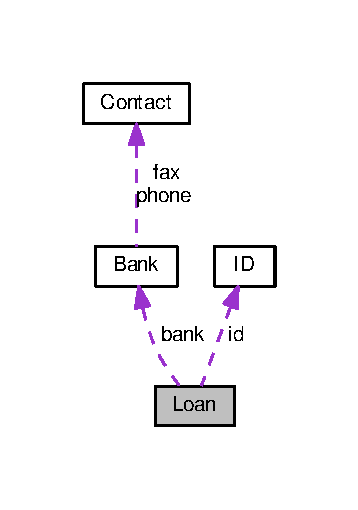
\includegraphics[width=172pt]{classLoan__coll__graph}
\end{center}
\end{figure}
\subsection*{Public Member Functions}
\begin{DoxyCompactItemize}
\item 
\hyperlink{classLoan_ac9837063879d5a4d21f288bdd5db6013}{Loan} ()
\item 
\hyperlink{classLoan_aefae6841fb1990b946ca473ff6a1ef8c}{Loan} (\hyperlink{classBank}{Bank} b, \hyperlink{classID}{I\+D} \hyperlink{classLoan_a77036ebdfea09fa00f2e6c5e1c7ee3c5}{id}, float \hyperlink{classLoan_a1cdd7876daa9a78ab7ac76cfdd17429e}{amount}, float \hyperlink{classLoan_a9b41857ab5a2bcc22bb877c14565071b}{rate}, int \hyperlink{classLoan_a9a132d11ff7a8126a1d7b556d03a4ea9}{term})
\item 
void \hyperlink{classLoan_a0536fb4faa0670d69afa6adf97ef161c}{set} ()
\begin{DoxyCompactList}\small\item\em T\+E\+S\+T diz This function sets the amounts. \end{DoxyCompactList}\item 
void \hyperlink{classLoan_a271b5df7e102eb82cb43c76029301fae}{display} ()
\begin{DoxyCompactList}\small\item\em a member function. \end{DoxyCompactList}\end{DoxyCompactItemize}
\subsection*{Private Attributes}
\begin{DoxyCompactItemize}
\item 
\hyperlink{classBank}{Bank} \hyperlink{classLoan_aa9d146c85226c7cd21d4963b1e826d69}{bank}
\item 
\hyperlink{classID}{I\+D} \hyperlink{classLoan_a77036ebdfea09fa00f2e6c5e1c7ee3c5}{id}
\item 
float \hyperlink{classLoan_a1cdd7876daa9a78ab7ac76cfdd17429e}{amount}
\item 
float \hyperlink{classLoan_a9b41857ab5a2bcc22bb877c14565071b}{rate}
\item 
int \hyperlink{classLoan_a9a132d11ff7a8126a1d7b556d03a4ea9}{term}
\end{DoxyCompactItemize}


\subsection{Detailed Description}
A Brief Desc? 

F\+I\+L\+E\+: \hyperlink{Loan_8h}{Loan.\+h} C\+L\+A\+S\+S P\+R\+O\+V\+I\+D\+E\+D\+: \hyperlink{classLoan}{Loan}

C\+O\+N\+S\+T\+R\+U\+C\+T\+O\+R\+S for the \hyperlink{classLoan}{Loan} class\+: \hyperlink{classLoan_ac9837063879d5a4d21f288bdd5db6013}{Loan()} Postcondition\+: \hyperlink{classBank}{Bank}, id, amount, rate, term are all set to zero \hyperlink{classLoan_aefae6841fb1990b946ca473ff6a1ef8c}{Loan(\+Bank b, I\+D id, float amount, float rate, int term)} Postcondition\+: bank is set per the \hyperlink{classBank}{Bank} criteria, id is set per the \hyperlink{classID}{I\+D}

M\+O\+D\+I\+F\+I\+C\+A\+T\+I\+O\+N M\+E\+M\+B\+E\+R F\+U\+N\+C\+T\+I\+O\+N\+S for the \hyperlink{classLoan}{Loan} class\+: void \hyperlink{classLoan_a0536fb4faa0670d69afa6adf97ef161c}{set()} Postcondition\+: bank, id, amount, rate, term are all set to legal terms as per the documentation for the respective classes by the user.

C\+O\+N\+S\+T\+A\+N\+T M\+E\+M\+B\+E\+R F\+U\+N\+C\+T\+I\+O\+N\+S for the \hyperlink{classLoan}{Loan} class\+: void \hyperlink{classLoan_a271b5df7e102eb82cb43c76029301fae}{display()} Precondition\+: bank, id, amount, rate, term have been set to legal terms as per the documentation for the respective classes. Postcondition\+: All values across all classes are out putted to the screen for the user to see

{\itshape N\+O\+T\+E} see \hyperlink{Contact_8h}{Contact.\+h} documentation as to why above needs to be true

V\+A\+L\+U\+E S\+E\+M\+A\+N\+T\+I\+C\+S for the Date class\+: Assignments and the copy constructor may be used with Card objects \begin{DoxyAuthor}{Author}
Landen Marchand 
\end{DoxyAuthor}


\subsection{Constructor \& Destructor Documentation}
\hypertarget{classLoan_ac9837063879d5a4d21f288bdd5db6013}{\index{Loan@{Loan}!Loan@{Loan}}
\index{Loan@{Loan}!Loan@{Loan}}
\subsubsection[{Loan}]{\setlength{\rightskip}{0pt plus 5cm}Loan\+::\+Loan (
\begin{DoxyParamCaption}
{}
\end{DoxyParamCaption}
)}}\label{classLoan_ac9837063879d5a4d21f288bdd5db6013}
Searches whatever 
\begin{DoxyParams}{Parameters}
{\em Name} & of an item wer are seeing \\
\hline
\end{DoxyParams}
\begin{DoxyReturn}{Returns}
What the hell this is 
\end{DoxyReturn}
\hypertarget{classLoan_aefae6841fb1990b946ca473ff6a1ef8c}{\index{Loan@{Loan}!Loan@{Loan}}
\index{Loan@{Loan}!Loan@{Loan}}
\subsubsection[{Loan}]{\setlength{\rightskip}{0pt plus 5cm}Loan\+::\+Loan (
\begin{DoxyParamCaption}
\item[{{\bf Bank}}]{b, }
\item[{{\bf I\+D}}]{id, }
\item[{float}]{amount, }
\item[{float}]{rate, }
\item[{int}]{term}
\end{DoxyParamCaption}
)}}\label{classLoan_aefae6841fb1990b946ca473ff6a1ef8c}


\subsection{Member Function Documentation}
\hypertarget{classLoan_a271b5df7e102eb82cb43c76029301fae}{\index{Loan@{Loan}!display@{display}}
\index{display@{display}!Loan@{Loan}}
\subsubsection[{display}]{\setlength{\rightskip}{0pt plus 5cm}void Loan\+::display (
\begin{DoxyParamCaption}
{}
\end{DoxyParamCaption}
)}}\label{classLoan_a271b5df7e102eb82cb43c76029301fae}


a member function. 

\hypertarget{classLoan_a0536fb4faa0670d69afa6adf97ef161c}{\index{Loan@{Loan}!set@{set}}
\index{set@{set}!Loan@{Loan}}
\subsubsection[{set}]{\setlength{\rightskip}{0pt plus 5cm}void Loan\+::set (
\begin{DoxyParamCaption}
{}
\end{DoxyParamCaption}
)}}\label{classLoan_a0536fb4faa0670d69afa6adf97ef161c}


T\+E\+S\+T diz This function sets the amounts. 



\subsection{Member Data Documentation}
\hypertarget{classLoan_a1cdd7876daa9a78ab7ac76cfdd17429e}{\index{Loan@{Loan}!amount@{amount}}
\index{amount@{amount}!Loan@{Loan}}
\subsubsection[{amount}]{\setlength{\rightskip}{0pt plus 5cm}float Loan\+::amount\hspace{0.3cm}{\ttfamily [private]}}}\label{classLoan_a1cdd7876daa9a78ab7ac76cfdd17429e}
\$ amount of the loan \hypertarget{classLoan_aa9d146c85226c7cd21d4963b1e826d69}{\index{Loan@{Loan}!bank@{bank}}
\index{bank@{bank}!Loan@{Loan}}
\subsubsection[{bank}]{\setlength{\rightskip}{0pt plus 5cm}{\bf Bank} Loan\+::bank\hspace{0.3cm}{\ttfamily [private]}}}\label{classLoan_aa9d146c85226c7cd21d4963b1e826d69}
\hypertarget{classLoan_a77036ebdfea09fa00f2e6c5e1c7ee3c5}{\index{Loan@{Loan}!id@{id}}
\index{id@{id}!Loan@{Loan}}
\subsubsection[{id}]{\setlength{\rightskip}{0pt plus 5cm}{\bf I\+D} Loan\+::id\hspace{0.3cm}{\ttfamily [private]}}}\label{classLoan_a77036ebdfea09fa00f2e6c5e1c7ee3c5}
Assume unique int in 3 int parts \hypertarget{classLoan_a9b41857ab5a2bcc22bb877c14565071b}{\index{Loan@{Loan}!rate@{rate}}
\index{rate@{rate}!Loan@{Loan}}
\subsubsection[{rate}]{\setlength{\rightskip}{0pt plus 5cm}float Loan\+::rate\hspace{0.3cm}{\ttfamily [private]}}}\label{classLoan_a9b41857ab5a2bcc22bb877c14565071b}
Annual interest rate \hypertarget{classLoan_a9a132d11ff7a8126a1d7b556d03a4ea9}{\index{Loan@{Loan}!term@{term}}
\index{term@{term}!Loan@{Loan}}
\subsubsection[{term}]{\setlength{\rightskip}{0pt plus 5cm}int Loan\+::term\hspace{0.3cm}{\ttfamily [private]}}}\label{classLoan_a9a132d11ff7a8126a1d7b556d03a4ea9}


The documentation for this class was generated from the following files\+:\begin{DoxyCompactItemize}
\item 
\hyperlink{Loan_8h}{Loan.\+h}\item 
\hyperlink{Loan_8cpp}{Loan.\+cpp}\end{DoxyCompactItemize}

\chapter{File Documentation}
\hypertarget{Bank_8cpp}{\section{Bank.\+cpp File Reference}
\label{Bank_8cpp}\index{Bank.\+cpp@{Bank.\+cpp}}
}
{\ttfamily \#include $<$iostream$>$}\\*
{\ttfamily \#include \char`\"{}Bank.\+h\char`\"{}}\\*
Include dependency graph for Bank.\+cpp\+:\nopagebreak
\begin{figure}[H]
\begin{center}
\leavevmode
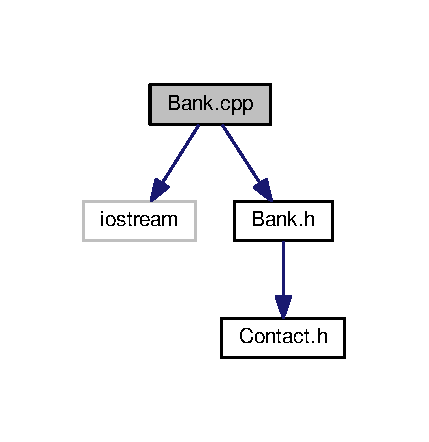
\includegraphics[width=206pt]{Bank_8cpp__incl}
\end{center}
\end{figure}

\hypertarget{Bank_8h}{\section{Bank.\+h File Reference}
\label{Bank_8h}\index{Bank.\+h@{Bank.\+h}}
}
{\ttfamily \#include \char`\"{}Contact.\+h\char`\"{}}\\*
Include dependency graph for Bank.\+h\+:\nopagebreak
\begin{figure}[H]
\begin{center}
\leavevmode
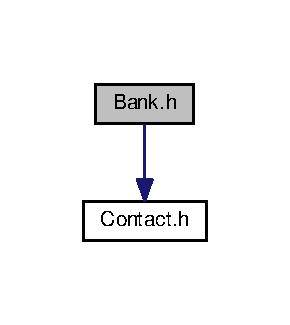
\includegraphics[width=139pt]{Bank_8h__incl}
\end{center}
\end{figure}
This graph shows which files directly or indirectly include this file\+:\nopagebreak
\begin{figure}[H]
\begin{center}
\leavevmode
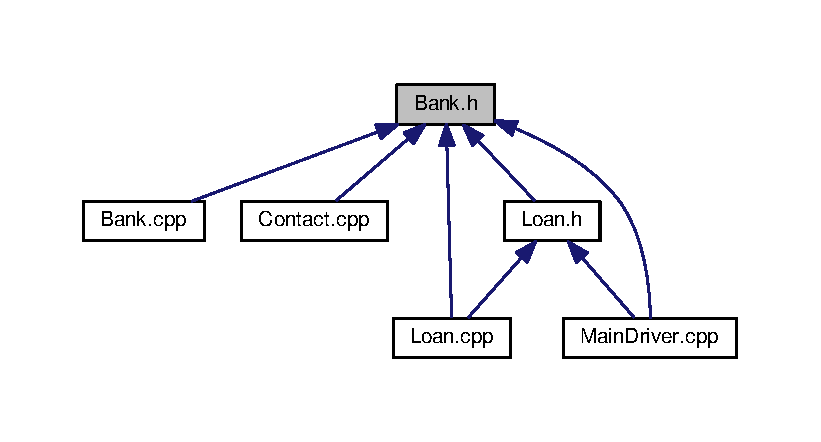
\includegraphics[width=350pt]{Bank_8h__dep__incl}
\end{center}
\end{figure}
\subsection*{Classes}
\begin{DoxyCompactItemize}
\item 
class \hyperlink{classBank}{Bank}
\end{DoxyCompactItemize}

\hypertarget{Contact_8cpp}{\section{Contact.\+cpp File Reference}
\label{Contact_8cpp}\index{Contact.\+cpp@{Contact.\+cpp}}
}
{\ttfamily \#include $<$iostream$>$}\\*
{\ttfamily \#include $<$cstdlib$>$}\\*
{\ttfamily \#include \char`\"{}Contact.\+h\char`\"{}}\\*
{\ttfamily \#include \char`\"{}Bank.\+h\char`\"{}}\\*
Include dependency graph for Contact.\+cpp\+:\nopagebreak
\begin{figure}[H]
\begin{center}
\leavevmode
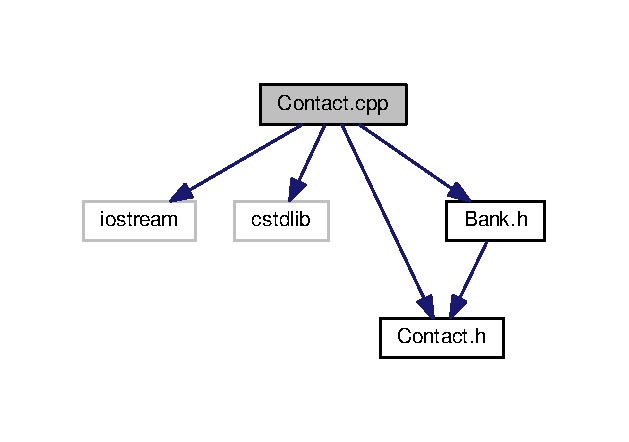
\includegraphics[width=302pt]{Contact_8cpp__incl}
\end{center}
\end{figure}

\hypertarget{Contact_8h}{\section{Contact.\+h File Reference}
\label{Contact_8h}\index{Contact.\+h@{Contact.\+h}}
}
This graph shows which files directly or indirectly include this file\+:\nopagebreak
\begin{figure}[H]
\begin{center}
\leavevmode
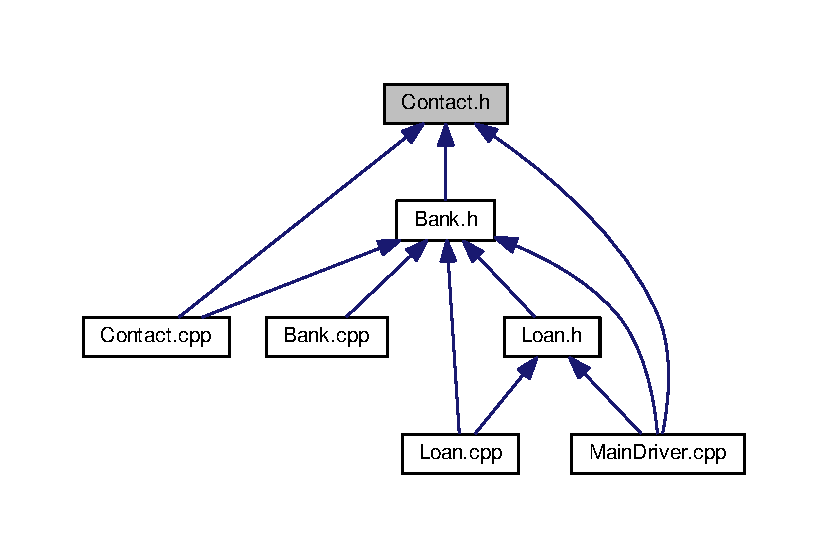
\includegraphics[width=350pt]{Contact_8h__dep__incl}
\end{center}
\end{figure}
\subsection*{Classes}
\begin{DoxyCompactItemize}
\item 
class \hyperlink{classContact}{Contact}
\end{DoxyCompactItemize}

\hypertarget{ID_8cpp}{\section{I\+D.\+cpp File Reference}
\label{ID_8cpp}\index{I\+D.\+cpp@{I\+D.\+cpp}}
}
{\ttfamily \#include $<$iostream$>$}\\*
{\ttfamily \#include $<$cassert$>$}\\*
{\ttfamily \#include \char`\"{}I\+D.\+h\char`\"{}}\\*
Include dependency graph for I\+D.\+cpp\+:\nopagebreak
\begin{figure}[H]
\begin{center}
\leavevmode
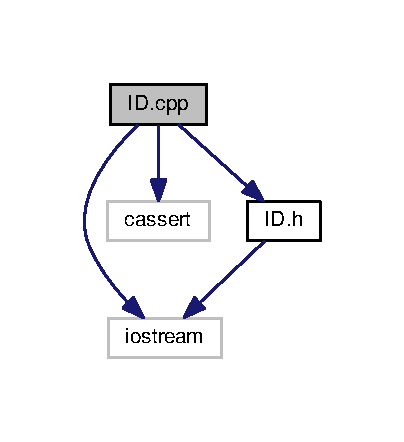
\includegraphics[width=194pt]{ID_8cpp__incl}
\end{center}
\end{figure}

\hypertarget{ID_8h}{\section{I\+D.\+h File Reference}
\label{ID_8h}\index{I\+D.\+h@{I\+D.\+h}}
}
{\ttfamily \#include $<$iostream$>$}\\*
Include dependency graph for I\+D.\+h\+:\nopagebreak
\begin{figure}[H]
\begin{center}
\leavevmode
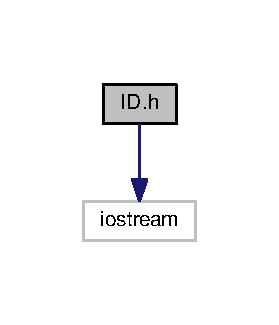
\includegraphics[width=134pt]{ID_8h__incl}
\end{center}
\end{figure}
This graph shows which files directly or indirectly include this file\+:\nopagebreak
\begin{figure}[H]
\begin{center}
\leavevmode
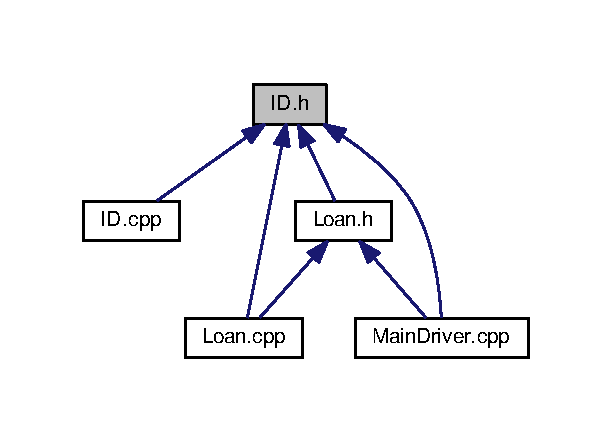
\includegraphics[width=294pt]{ID_8h__dep__incl}
\end{center}
\end{figure}
\subsection*{Classes}
\begin{DoxyCompactItemize}
\item 
class \hyperlink{classID}{I\+D}
\end{DoxyCompactItemize}

\hypertarget{Loan_8cpp}{\section{Loan.\+cpp File Reference}
\label{Loan_8cpp}\index{Loan.\+cpp@{Loan.\+cpp}}
}
{\ttfamily \#include \char`\"{}Loan.\+h\char`\"{}}\\*
{\ttfamily \#include \char`\"{}Bank.\+h\char`\"{}}\\*
{\ttfamily \#include \char`\"{}I\+D.\+h\char`\"{}}\\*
{\ttfamily \#include $<$iostream$>$}\\*
{\ttfamily \#include $<$cassert$>$}\\*
Include dependency graph for Loan.\+cpp\+:\nopagebreak
\begin{figure}[H]
\begin{center}
\leavevmode
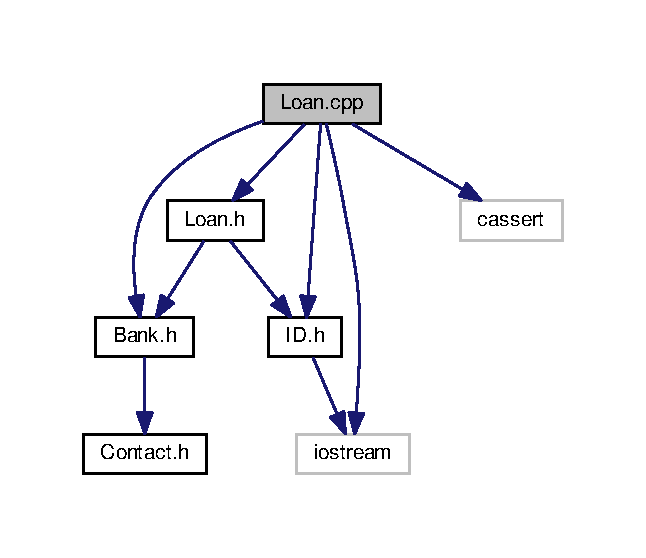
\includegraphics[width=310pt]{Loan_8cpp__incl}
\end{center}
\end{figure}

\hypertarget{Loan_8h}{\section{Loan.\+h File Reference}
\label{Loan_8h}\index{Loan.\+h@{Loan.\+h}}
}
{\ttfamily \#include \char`\"{}Bank.\+h\char`\"{}}\\*
{\ttfamily \#include \char`\"{}I\+D.\+h\char`\"{}}\\*
Include dependency graph for Loan.\+h\+:\nopagebreak
\begin{figure}[H]
\begin{center}
\leavevmode
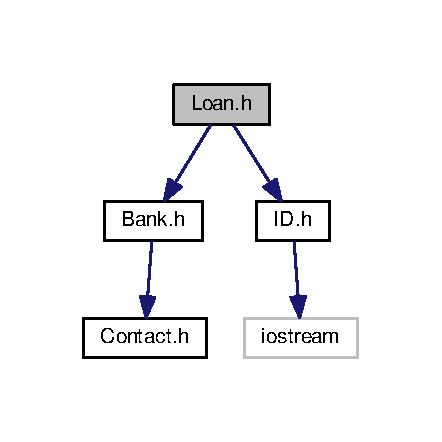
\includegraphics[width=212pt]{Loan_8h__incl}
\end{center}
\end{figure}
This graph shows which files directly or indirectly include this file\+:\nopagebreak
\begin{figure}[H]
\begin{center}
\leavevmode
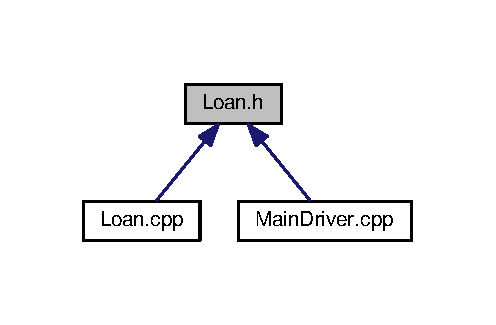
\includegraphics[width=238pt]{Loan_8h__dep__incl}
\end{center}
\end{figure}
\subsection*{Classes}
\begin{DoxyCompactItemize}
\item 
class \hyperlink{classLoan}{Loan}
\begin{DoxyCompactList}\small\item\em A Brief Desc? \end{DoxyCompactList}\end{DoxyCompactItemize}

\hypertarget{MainDriver_8cpp}{\section{Main\+Driver.\+cpp File Reference}
\label{MainDriver_8cpp}\index{Main\+Driver.\+cpp@{Main\+Driver.\+cpp}}
}
{\ttfamily \#include $<$iostream$>$}\\*
{\ttfamily \#include \char`\"{}Bank.\+h\char`\"{}}\\*
{\ttfamily \#include \char`\"{}Contact.\+h\char`\"{}}\\*
{\ttfamily \#include \char`\"{}I\+D.\+h\char`\"{}}\\*
{\ttfamily \#include \char`\"{}Loan.\+h\char`\"{}}\\*
Include dependency graph for Main\+Driver.\+cpp\+:\nopagebreak
\begin{figure}[H]
\begin{center}
\leavevmode
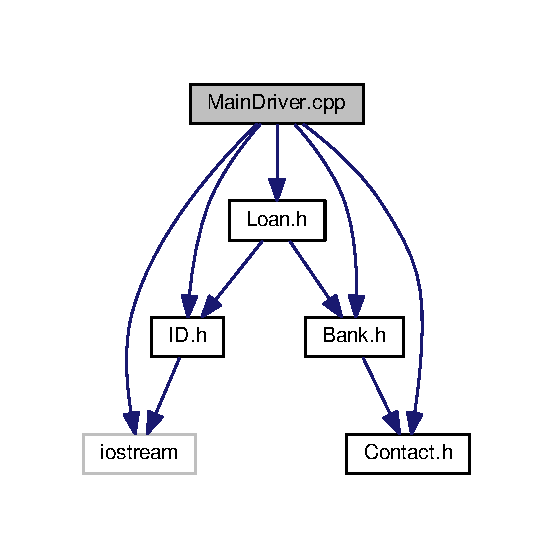
\includegraphics[width=266pt]{MainDriver_8cpp__incl}
\end{center}
\end{figure}
\subsection*{Functions}
\begin{DoxyCompactItemize}
\item 
int \hyperlink{MainDriver_8cpp_ae66f6b31b5ad750f1fe042a706a4e3d4}{main} ()
\end{DoxyCompactItemize}


\subsection{Function Documentation}
\hypertarget{MainDriver_8cpp_ae66f6b31b5ad750f1fe042a706a4e3d4}{\index{Main\+Driver.\+cpp@{Main\+Driver.\+cpp}!main@{main}}
\index{main@{main}!Main\+Driver.\+cpp@{Main\+Driver.\+cpp}}
\subsubsection[{main}]{\setlength{\rightskip}{0pt plus 5cm}int main (
\begin{DoxyParamCaption}
{}
\end{DoxyParamCaption}
)}}\label{MainDriver_8cpp_ae66f6b31b5ad750f1fe042a706a4e3d4}

%--- End generated contents ---

% Index
\newpage
\phantomsection
\addcontentsline{toc}{chapter}{Index}
\printindex

\end{document}
